\documentclass[11pt, oneside, a4paper, titlepage]{article}

% We use the 'tcolorbox' package to create most of the formatting.
\usepackage[most]{tcolorbox}

% We use the 'geometry' package to set the margins to be exactly what we want.
% In this case 2.54 cm (1 inch) all around, to match those that MS word uses by default.
% Note that we use different margins at the top and bottom
% to take account of the custom header and footer that we are using.
\usepackage{geometry}
\geometry{
    a4paper,
    left=0.1cm,
    right=0.1cm,
    top=0.1cm,
    bottom=0.1cm
}

\usepackage{hyperref}

\definecolor{titleBack}{RGB}{54, 53, 55}
% original titleBack {0, 66, 21}
% Jet {54, 53, 55}
% Melon {253, 179, 169}
% Deep Taupe {124, 97, 108}
% Independence {72, 77, 109}
% Indigo Dye {34, 72, 112}
% Dark Purple {65, 34, 52}

\definecolor{lightPurple}{RGB}{242, 235, 251}

\definecolor{someOrange}{RGB}{255, 192, 92}

\usepackage{titlesec}

\titleformat{\section}
{\LARGE}
{}
{-1em}
{\bfseries}[]

\titleformat{\subsection}
{\Large}
{}
{0em}
{\bfseries}[]

\titleformat{\subsubsection}[runin]
{}
{}
{0em}
{\bfseries}[ ---]

\title{Atharva Pardeshi}
\date{}

\newcommand\experienceVSpace{\vspace{-0.1cm}}
\newcommand\skillsVSpace{\vspace{-0.3cm}}

\begin{document}

\tcbset{colframe=gray!95!black,colback=titleBack,arc=0mm}
\begin{tcolorbox}
  % \begin{minipage}{4.5cm}
  %   \hspace*{-0.2cm}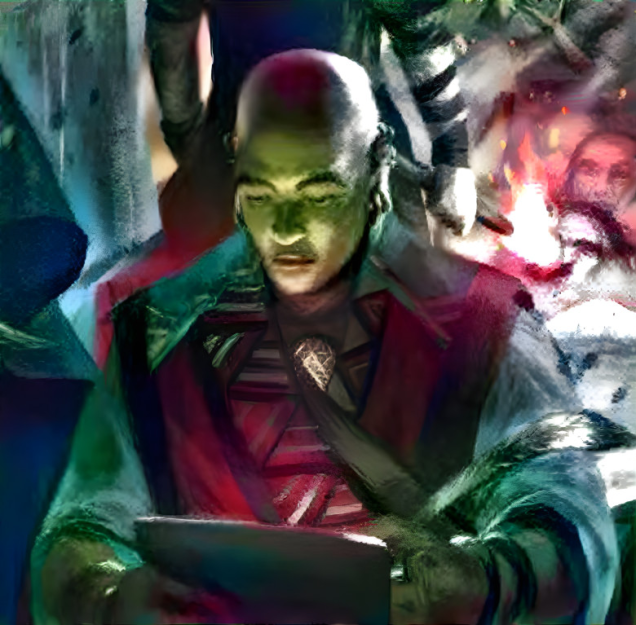
\includegraphics[width=4cm]{spooky-sazed.png}
  % \end{minipage}
  \begin{minipage}{4.5cm}
    \subsection{\textcolor{white}{Contact}}
    \textcolor{white}{Email-}\href{mailto:atharva.exe@gmail.com}{\underline{\textcolor{white}{atharva.exe@gmail.com}}} \\
    \textcolor{white}{Website-}\href{https://atharva-pardeshi.netlify.app}{\underline{\textcolor{white}{atharva-pardeshi.netlify.app}}} \\
    \textcolor{white}{GitHub-}\href{https://github.com/SazedWorldbringer}{\underline{\textcolor{white}{SazedWorldbringer}}} \\
    \textcolor{white}{Linkedin-}\href{https://linkedin.com/in/atharvapardeshi}{\underline{\textcolor{white}{atharvapardeshi}}} \\
  \end{minipage}
  \begin{minipage}{15cm}
    \begin{center}
      \Huge{\textcolor{white}{Atharva Pardeshi}} \\
      \vspace*{0.5cm}
      \Large{\textcolor{white}{\textit{Software Developer}}}
    \end{center}
  \end{minipage}
\end{tcolorbox}

\tcbset{colframe=white,colback=white,arc=0mm}
\begin{tcolorbox}
  \begin{minipage}[t]{8cm}
    \vspace*{-0.5cm}
    \begin{tcolorbox}[grow to left by=0.6cm,colback=gray!25,colframe=white]

      \section*{Profile}
      \begin{itemize}
        \item{
      A self-taught software developer,
      who believes great software is easy to read,
      maintain and debug.
          }
        \item{
      I believe coding standards and best practices are absolutely critical
      for the long-term success of any software project.
          }
        \item{
      I see teamwork, open communication and compassion
      as the most key values for working together.
          }
        \item{
      Empathy, calm, and optimism
      help me deal well with everyday challenges and pressure.
        }
      \item{
      I strive to be curious, humble and ready to adapt
      believing those are the most important qualities to have
      for succeeding in the tech industry.
        }
      \end{itemize}


      \section*{Skills}
        \subsubsection{Programming, Scripting and Markup Languages}
        C, Lisp, JavaScript, Python, Sql, {\LaTeX}, HTML, CSS, SASS/LESS, Markdown
        \skillsVSpace
        \subsubsection{Libraries/Frameworks}
        React.js, Next.js, Node.js, TailwindCSS, Chakra UI, Material UI

        \skillsVSpace
        \subsubsection{Work Flow}
        (Neo)Vim, VSCode, Git, GitHub, Terminal, Linux/Windows

        \skillsVSpace
        \subsubsection{Computer Science}
        Algorithms \& Data Structures, 

      \section*{Interests}
      \begin{itemize}
        \item{Contributing to Open Source projects}
        \item{Buiding, breaking and fixing software}
        \item{Reading Science fiction and Fantasy, Technical books}
      \end{itemize}
    \end{tcolorbox}
  \end{minipage}
  \begin{minipage}[t]{11cm}
    \vspace*{-0.5cm}
    \begin{tcolorbox}[grow to right by=0.75cm,colframe=white,colback=white]
      \section*{Experience}
      \begin{itemize}
        \item
        {
          \textbf{Jammming} \\
          \textit{A playlist app made with the Spotify API} \\
          \textit{Live-  \href{https://jammming-sazed.netlify.app}{\underline{jammming-sazed.netlify.app}} | \href{https://github.com/SazedWorldbringer/codecademy-jammming}{\underline{GitHub Repo}}} \\
          \vspace*{-0.7cm}
          \begin{itemize}
            \item Connects to user's Spotify account.
              \experienceVSpace
            \item {Allow users to:
                \vspace{-0.2cm}
                \begin{enumerate} 
                  \item{Search the Spotify library,}
                    \vspace{-0.2cm}
                  \item{Create custom playlists,} 
                    \vspace{-0.2cm}
                  \item{And save the playlist to their Spotify accounts.}
                \end{enumerate}
              }
          \end{itemize}
        }

        \item
        {
          \textbf{Project Title} \\
          \textit{Project Description} \\
          \textit{Live- \href{url}{\underline{project name}} | \href{https://github.com/SazedWorldbringer}{\underline{GitHub Repo}}} \\
          \vspace*{-0.7cm}
          \begin{itemize}
            \item Project line 1
              \experienceVSpace
            \item Project line 1
              \experienceVSpace
            \item Project line 1
          \end{itemize}
        }

        \item
        {
          \textbf{NinjaFood} \\
          \textit{A recipe search app, where you can look up recipes and save to favorites} \\
          \textit{Live- \href{https://ninja-food-repo.netlify.app}{\underline{ninja-food-repo.netlify.app}} | \href{https://github.com/SazedWorldbringer/ninjafood}{\underline{GitHub Repo}}} \\
          \vspace*{-0.7cm}
          \begin{itemize}
            \item Fetch recipes from TheMealDB API.
              \experienceVSpace
            \item Like a recipe by saving it to localstorage.
              \experienceVSpace
            \item Implemented the UI using TailwindCSS.
          \end{itemize}
        }

        \item
        {
          \textbf{Prime Finance} \\
          \textit{Landing page for a financing application} \\
          \textit{Live- \href{https://prime-finance.netlify.app}{\underline{prime-finance.netlify.app}} | \href{https://github.com/SazedWorldbringer/prime-finance-react}{\underline{GitHub Repo}}} \\
          \vspace*{-0.7cm}
          \begin{itemize}
            \item Landing page with a nice, minimal UI
              \experienceVSpace
            \item Implemented the UI using TailwindCSS
              \experienceVSpace
            \item Used react-type-animation for the typing animation
          \end{itemize}
        }

        \item
        {
          \textbf{Project Title} \\
          \textit{Project Description} \\
          \textit{Live- \href{url}{\underline{project name}} | \href{https://github.com/SazedWorldbringer}{\underline{GitHub Repo}}} \\
          \vspace*{-0.7cm}
          \begin{itemize}
            \item Project line 1
              \experienceVSpace
            \item Project line 1
              \experienceVSpace
            \item Project line 1
          \end{itemize}
        }
      \end{itemize}
      \section*{Education}
      \begin{itemize}
        \item
        {
          \textbf{KTHM College, Nashik} \\
          \textit{Junior College -- 12th HSC Science} \\
          \textit{2019 - 2021} \\
        }
        % \item
        % {
        %   \textbf{Another University} \\
        %   \textit{A masters degree} \\
        %   \textit{2004 - 2009} \\
        % }
        % \item
        % {
        %   \textbf{Some University} \\
        %   \textit{Bachelors degree} \\
        %   \textit{2004 - 2009} \\
        % }
      \end{itemize}
    \end{tcolorbox}
  \end{minipage}
\end{tcolorbox}

\end{document}
